\subsection{Catmull-Clark-Unterteilung}
Im Zuge des Projektes wurde der Catmull-Clark-Algorithmus für Unterteilungsflächen umgesetzt. 
Darauf soll in den folgenden Unterkapiteln genauer eingangen werden. 
Zuerst wird der allgemeine Fall betrachtet. 
Anschließend die Regelungen für scharfe Kanten und spitze Punkte. 
Abschließend wird noch kurz auf die Limitpunkte eingegangen.

\subsubsection{Allgemeiner Algorithmus}
Bei dem Algorithmus werden die Flächen des Meshes unterteilt. 
Dabei entsteht für jeden existierenden Punkt, jede Kante und jede Fläche ein neuer Punkt.
Dies funktioniert für beliebige Topologien. 
Nach der ersten Iteration des Algorithmus gibt es im Mesh nur noch Flächen mit Valenz vier.
Des Weiteren enstehen nach der ersten Iteration nurnoch Punkte mit Valenz vier. 
Die Anzahl der irregulären Punkte \emph{nach} der ersten Iteration bleibt gleich.

Die neuen Punkte werden nach folgenden Regeln gebildet:\\
\begin{itemize}
\item Ein neuer Flächenpunkt errechnet sich aus dem Mittel der die Fläche umschließenden Punkte.
\item Ein neuer Kantenpunkt wird aus dem Mittel der neuen Flächenpunkten und der angrenzenden Punkte der Kante gebildet.
\item Neue Eckpunkte werden aus den neuen, angrenzenden Flächenpunkten, den inzidenten Punkten und dem alten Eckpunkt errechnet.
\end{itemize}

Im folgenden wird auf die genauen Berechnungen eingangen.

\paragraph{Flächenpunkte}
\begin{figure}[htpb]
\centering
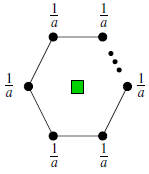
\includegraphics[scale=0.8]{content/pictures/facepoints.png}
\caption{Berechnung der Flächenpunkte}
\label{fig:facepoints}
\end{figure}

In Abb.~\ref{fig:facepoints} wird die Berechnung der neuen Flächenpunkte(grün) dargestellt. Die Variable \emph{a} bezeichnet die Flächenvalenz der jeweiligen Fläche.

\paragraph{Kantenpunkte}
\begin{figure}[htpb]
\centering
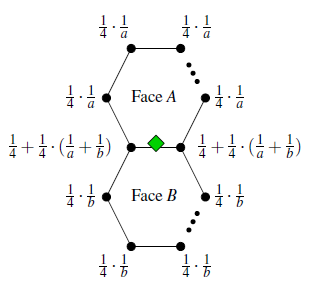
\includegraphics[scale=0.8]{content/pictures/edgepoints.png}
\caption{Berechnung der Kantenpunkte}
\label{fig:edgepoints}
\end{figure}

Die Kantenpunkte(grün) werden wie in Abb. ~\ref{fig:edgepoints} ermittelt. Die Variable \emph{a} bezeichnet die Flächenvalenz der Fläche A und die Variable \emph{b} entsprechend für Fläche B. Zu beachten ist hier der Spezialfall in Kap.~\ref{sec:sharpEdge}.

\paragraph{Eckpunkte}
\begin{figure}[htpb]
\centering
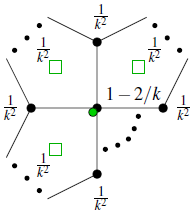
\includegraphics[scale=0.8]{content/pictures/vertexpoints.png}
\caption{Berechnung der Eckpunkte}
\label{fig:vertexpoints}
\end{figure}

Die neuen Eckpunkte ergeben sich durch Anteile der neuen Flächenpunkte und der alten, inzidenten Eckpunkte, wie in Abb.~\ref{fig:vertexpoints} dargestellt. Hierbei bezeichnet \emph{k} die Punktvalenz.

\subsubsection{Scharfe Kanten und spitze Punkte}
\label{sec:sharpEdge}
Eine scharfe Kante verwendet gesonderte Regeln um beim Unterteilen andere Ergebnisse zu erzielen. Dies begründet sich darin, dass bei der Berechnung nur die inzidenten Eckpunkte betrachtet werden. Es entstehen sichtbare Knicke im Mesh. \\

Ein spezieller Einsatzbereich der scharfen Kanten ist die Umrandung von Löchern im Mesh. Der Einsatz scharfer Kanten verhindert hierbei ein Anwachsen der Lochgröße.
\begin{figure}[tpb]
\centering
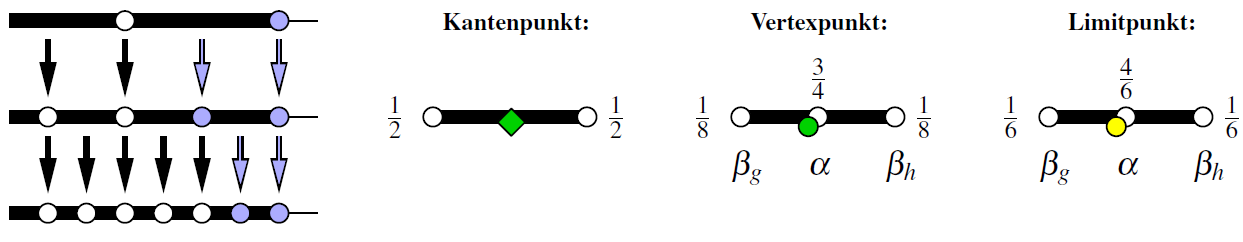
\includegraphics[width=\columnwidth]{content/pictures/sharpLimit.png}
\caption{Berechnung der scharfen Kanten mit Limitpunkten}
\label{fig:sharpLimit}
\end{figure}
Die Kantenpunkte und Eckpunkte, die auf einer scharfen Kante liegen, errechnen sich mit den in Abb.~\ref{fig:sharpLimit} gezeigten Verhältnissen. 

Ein spitzer Punkt erhält bei der Unterteilung durch Catmull-Clark seine Ursprungsposition.

\subsubsection{Limitpunkte}
Durch den Einsatz des Catmull-Clark Algorithmus schrumpft das unterteilte Mesh. Nach unendlich vielen Iterationen konvergiert das Mesh gegen eine Limitfläche. 
Für einen Punkt des Meshes lässt sich sein zugehöriger Punkt auf der Limitfläche bestimmen, die dazu benötigten Regeln heißen Limitpunktregeln.
\begin{figure}[htpb]
\centering
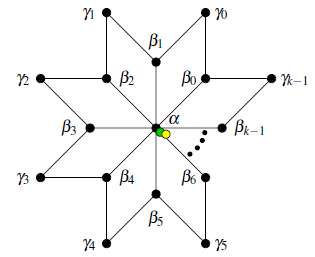
\includegraphics[scale=0.7]{content/pictures/limit.png}
\caption{Berechnung der Limitpunkte}
\label{fig:limit}
\end{figure}

Abb.~\ref{fig:limit} zeigt einen Ausschnitt aus einem Vierecksmesh.
Die Variablen $\alpha$ , $\beta$ und $\gamma$ beschreiben den Eckpunkt, seine inzidenten Eckpunkte und die Eckpunkte in Zweier-Nachbarschaft.  

In den Limitpunkt gehen die genannten Komponenten zu folgenden Verhältnissen ein. Hierbei bezeichnet \emph{k} die Punktvalenz und \emph{i} den i-ten inzidenten Punkt bzw. Punkt in Zweier-Nachbarschaft.
\begin{equation}
\alpha = 1-\dfrac{5}{k+5}\\
\beta_i = \dfrac{4}{(k+5)k}\\
\gamma_i = \dfrac{1}{(k+5)k}
\end{equation}

An scharfen Kanten gelten für die Berechnung von Limitpunkten die in Abb.~\ref{fig:sharpLimit} gezeigten Verhältnisse.

\subsection{Punktglättung}
Bei der Punktglättung werden alle Punkten, der zu einem Punkt inzidenten Flächen, mit dem Ursprungspunkt addiert. 
Aus dem Mittel ergibt sich der geglättete Punkt. 
Zwischen dem Ursprungspunkt und dem geglätteten Punkt kann man nun per Interpolation eine beliebige Glättungsstufe erhalten.

\subsection{Löschen von Punkten, Kanten und Flächen}
Im folgenden wird die Funktion, Punkte, Kanten und Flächen zu löschen näher betrachtet.
Insbesondere wird kurz auf Besonderheiten bei den einzelnen Verfahren hingewiesen.
\subsubsection{Löschen von Punkten}
Das Löschen von Punkten ist der schwierigste Fall beim Löschen. Hierbei müssen einige Schritte unternommen werden und auf einige Spezialfälle geachtet werden. 
Allgemein betrachtet muss folgendes geschehen:
\begin{itemize}
\item Der ausgewählte Punkt muss entfernt werden.
\item Alle inzidenten Kanten müssen entfernt werden.
\item Alle inzidenten Flächen müssen entfernt werden.
\item Die inzidenten Eckpunkte zeigen nicht mehr auf die entfernten Kanten.
\item Die Valenz der inzidenten Eckpunkte muss angepasst werden.
\item An der entsprechenden Stelle entstehen ein oder mehrere Löcher.
\item Die HalfEdge-Datenstruktur an der entsprechenden Stelle muss aktualisiert werden. Dabei muss die Konsistenz trotz entfernter Kanten und eines oder mehrerer neuer Löcher erhalten bleiben.
\end{itemize}

\subsubsection{Löschen von Kanten}
Das Löschen von Kanten ist dem Löschen eines Punktes recht ähnlich.
\begin{itemize}
\item Die entsprechende Kante (und damit die unterliegenden Halfedges) müssen entfernt werden. 
\item Die inzidenten Flächen werden entfernt und durch ein oder mehrere Löcher ersetzt.
\item Die Valenz der inzidenten Punkte muss entsprechend angepasst werden.
\item Die HalfEdge-Datenstruktur muss wie oben aktualisiert werden, um die Konsistenz zu erhalten.
\end{itemize}

\subsubsection{Löschen von Flächen}
Das Löschen einer Fläche ist der einfachste Fall.
Hierbei wird lediglich die Fläche durch ein Loch ersetzt und die HalfEdge-Datenstruktur mit scharfen Kanten versehen.
